In this section we'll present and analyze the main components (and their sub-parts) in which our system is divided and we'll explain the relations between them.
		
\subsection{Application Server}
\label{subsect:Application Server}
	\begin{figure}[H]
		\begin{center}
			\hspace*{-60pt}
			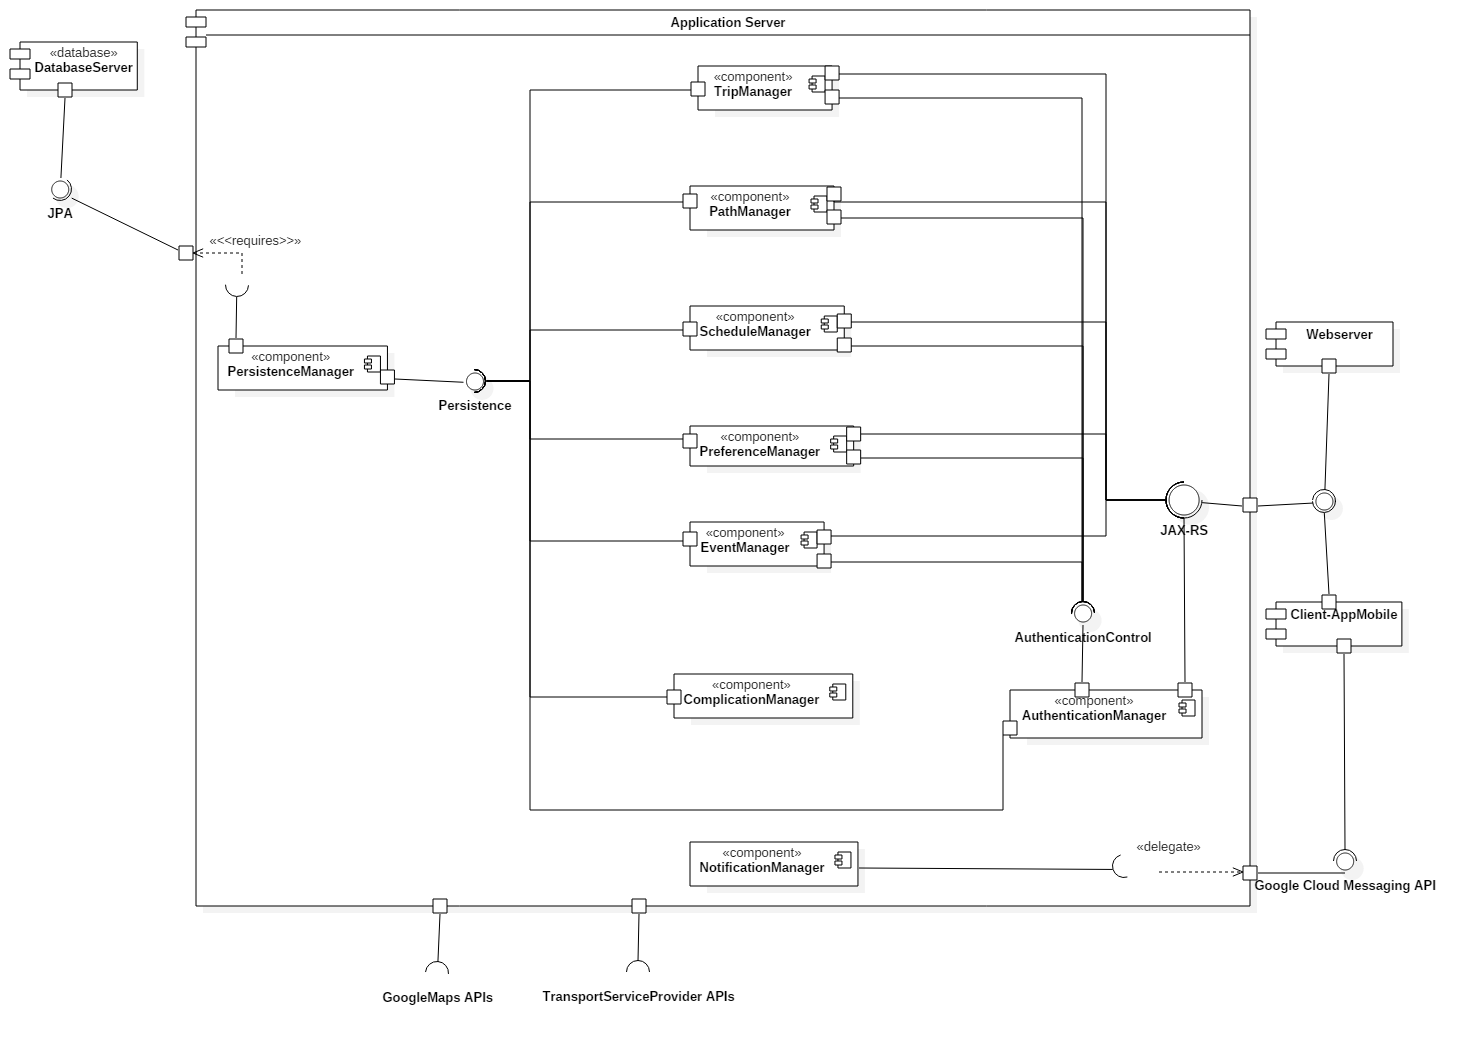
\includegraphics[scale=0.4]{ApplicationServer.png}
		\end{center}
		\caption{The components of the Application Server}
	\end{figure}
	The application server must handle the whole business logic of the application and the connection with the data layer. It must expose all the required functionalities to the users. It also has to interact with external systems. \\ \\
The main components of the Application Server are:
\begin{itemize}
	\item \textbf{AuthenticationManager:} This module will manage the user registration, the user login and it will be involved in any user request to the application server in order to check if the request comes from an authorized device;
	\item \textbf{CalendarManager:} This subsystem will manage all calendar-related functionalities of Travlendar+'s system, its structure will be better explained in the dedicated section below, along with a schema of its internal components;
	\item \textbf{TripManager:} This module will provide the logic needed to arrange the user trips; to do so, this module will interact with external systems of Transport service providers, in order to allow the user to buy public transportation tickets or to locate the nearest vehicle of a sharing system, when those travel means are involved in the user's travel path;
	\item \textbf{ComplicationManager:} This module will periodically checks if the travels that are close in time are still feasible. To do so it will interact with external systems of Transport service providers to gain information about strikes, with open weather APIs to obtain information about the weather and with \textit{Google Maps APIs} to obtain information about the traffic. If this module detects that a travel is no more feasible, it will charge the \textit{NotificationManager} to warn the involved user;
	\item \textbf{NotificationManager:} This module will serve as a gateway to all the notifications to be sent, from others modules, to the user's mobile devices. To do so it will use the \textit{Google Cloud Messaging APIs} in order to ensure a transparent interface with both IOS and Android devices;
	\item \textbf{PersistenceManager:} This module will provide transparent access to the database functionalities from all the others modules. All system database-related functionalities must be developed inside this module. If some users have inserted one or more periodic events, this module will handle their propagation in the time (see also section \ref{subsect:Periodic events}); 
\end{itemize}

\subsubsection{Calendar Manager}
\label{subsubsect:Calendar Manager}
\begin{figure}[H]
	\begin{center}
		\hspace*{-60pt}
		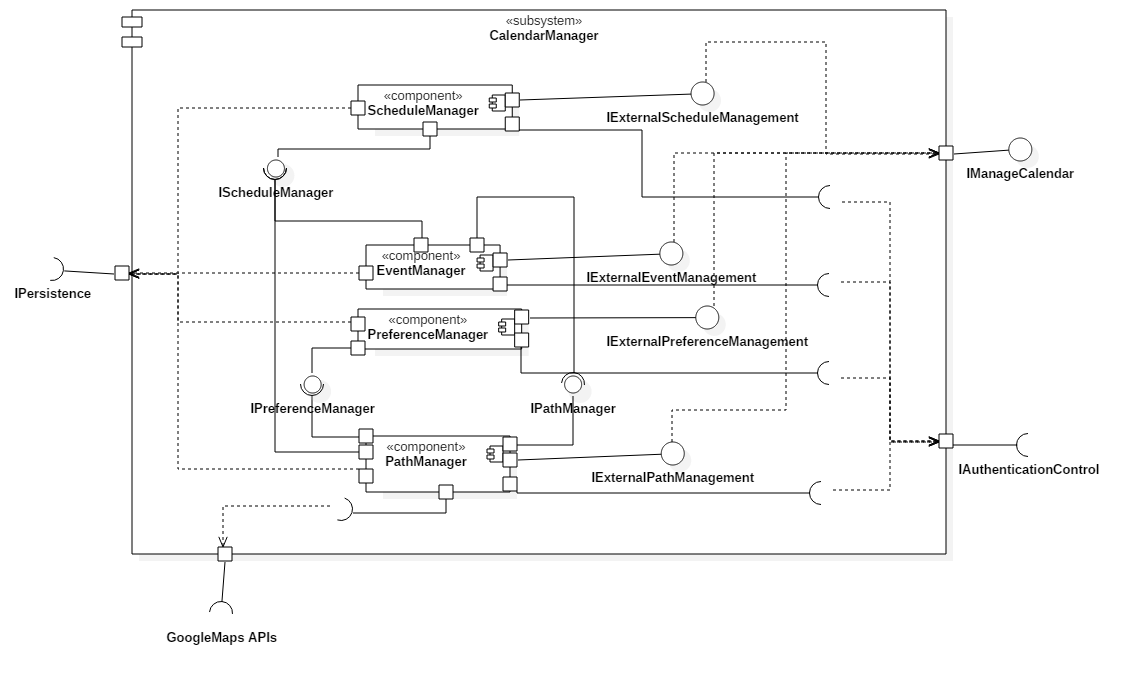
\includegraphics[scale=0.5]{CalendarSubsystem.png}
	\end{center}
	\caption{The components of the CalendarManager subsystem}
\end{figure}
	This subsystem will implement almost all the core functionalities of our system.\\ It is composed of four main components:
	\begin{itemize}
		\item \textbf{PathManager:} This module will manage the user travels computation, after the insertion or the modification of an event, or also after a specific user requests to change a selected path. It will compute the feasible paths through proprietary internal logic and the involvement of \textit{Google Maps API}. It will also interact with the \textit{PreferenceManager} in order to obtain the information needed to guarantee that the user preferences are respected in every proposed path;
		\item \textbf{EventManager:} This module will manage the insertion, deletion and modification of the events into the user calendar. It will interact with the \textit{ScheduleManager} in order to find out if an event does overlap with other events. When an event is created it will involve the \textit{PathManager} in order to provide feasible paths to reach the inserted events. It will also handle insertion, deletion and modification of the flexible breaks;
		\item \textbf{ScheduleManager:} This module will manage the event's scheduling functionalities: it is able to check if an event overlaps with other events and to guarantee that the flexible breaks are respected. It will also check that the user's travels do not overlap with other events. When an event overlaps with another one, it will put in a separate list of non scheduled events and it will manage the user's requests of rescheduling these events.
		\item \textbf{PreferenceManager:} This module will offer all the functionalities needed to insert, modify and delete the user's event profiles. It will also interact with the module that has to apply the event profiles in order to compute the travel paths (\textit{PathManager}).
	\end{itemize}
	
\subsection{Database}
\label{subsect:Database}
	The \textit{Database Server} must manage the insertion, deletion and modification on data inside his secondary memory. This layer must guarantee ACID distributed transactions.\\
	Since we've already provided an exhaustive description of the model of the data to be memorized into the database (\textbf{see Section 2.2.1 of RASD document}) we will not insert here another diagram.\\
	Nonetheless some small additions must be made to that diagram: in the tables it must be added a time-stamp field in order to handle the update of the mobile Application's Local Database with only the actual changes in the database (detailed explanation in section \ref{subsect:Local database update}), it must be also memorized an additional table that will store all the IDs of the devices connected to an account and the relative univocal code associated with them (detailed explanation in section \ref{subsect:Authentication}).	

\subsection{Web Server}
\label{subsect:Web Server}
	The web server layer connects the users that want to use Travlendar+ through a web browser with the Application Server. \newline
	The main functions to be implemented in this layer are basically web interfaces.
	The only logic in this layer is used to embed a map into the relative web page and to draw the paths the user must travel to reach his events. To do so the web browser will interact with\textit{ Google Polylines APIs}.
	The presentation will be handled by the \textit{JavaServerPages} component that will be implemented using JSP pages. The interaction with the Application server and with the maps APIs will be handled by the \textit{WebController} module.
	
\begin{figure}[H]
\begin{center}
		\hspace*{-0pt}
		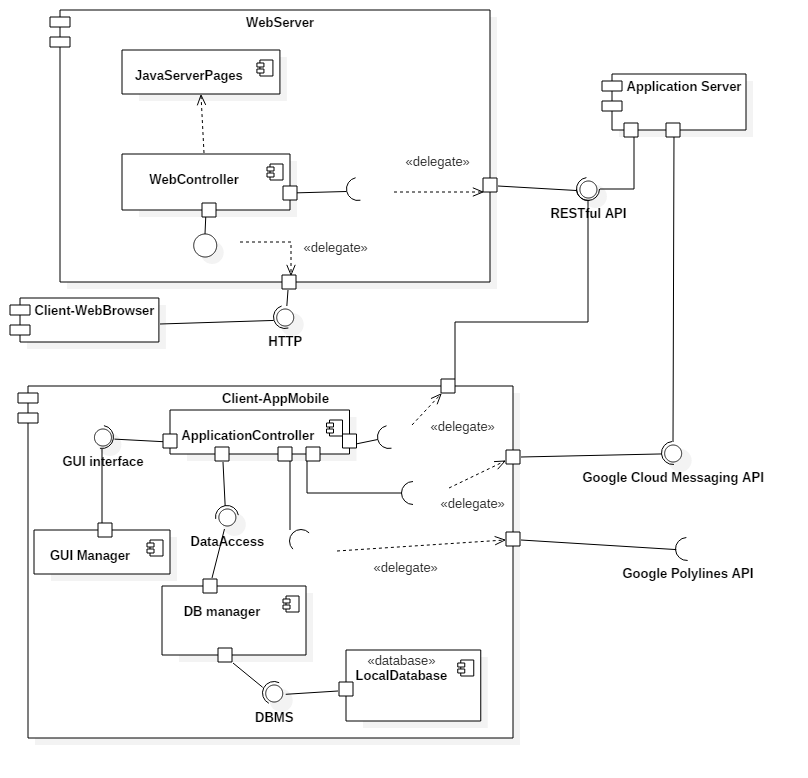
\includegraphics[scale=0.5]{Client_and_web_server.png}
\end{center}
\caption{The components of the web server, of the client app and of the client browser}
\end{figure}

\subsection{App Mobile}
\label{subsect:App Mobile}
	The layer that connects the users that want to use Travlendar+ through their mobile devices with the Application Server.
	To do so it uses three main modules: 
	\begin{itemize}
	\item the \textit{GUIManager}: it handles all the presentation functionalities of the app;
	\item the \textit{DBManager}: it handles all the users data, such as events and some information about travels duration, in order to enable the user to use some of the app functionalities even when he does not have access to an Internet connection (see also the E-R diagram in image \ref{fig:localDB});
	\item the \textit{ApplicationController}: it handles the interaction with the server, using the inputs provided by the users through the \textit{GUIManager} and also requesting data manipulation operations in the local app database with the information received from the server (in order to perform an update of the \textit{Local Database}).
	\end{itemize}
	The application controller will also handle the notifications received and it will interact with \textit{Google Polylines APIs} for mobile devices in order to to draw the paths the user must travel to reach his events and provide GPS path following functionalities.
\begin{figure} [H]
	\begin{center}
		\hspace*{-10pt}
		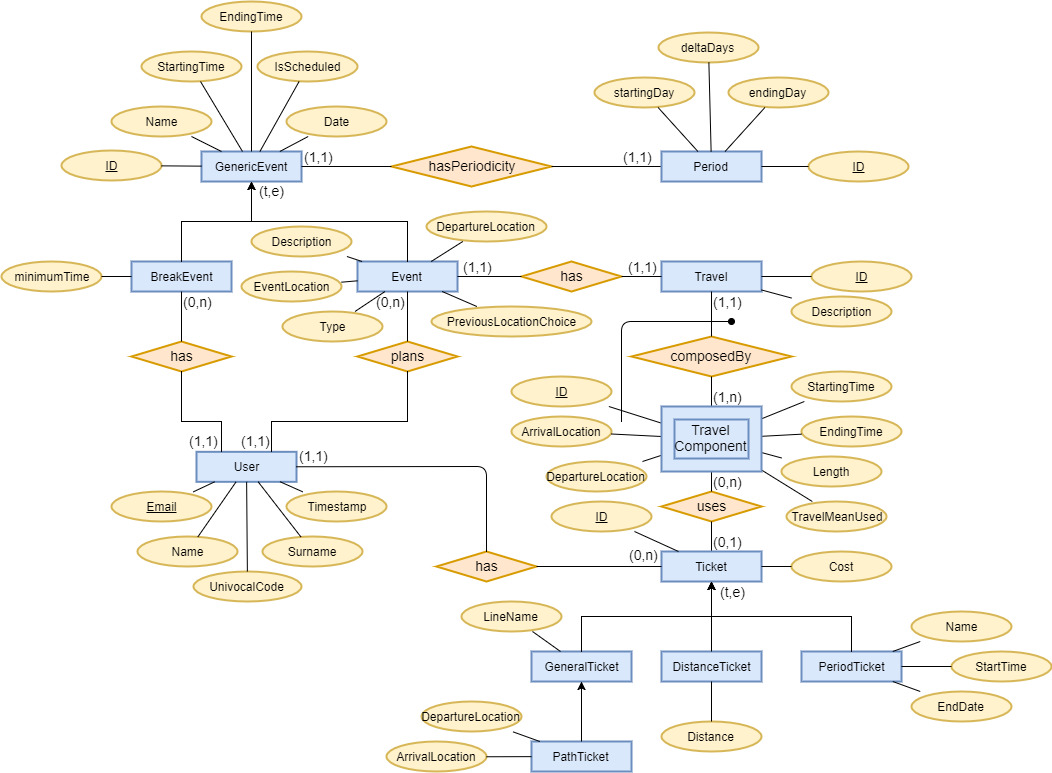
\includegraphics[scale=0.4]{er_diagram.png}
	\end{center}
	\caption{E-R diagram representing the mobile app Local Database data structure.}
	\label{fig:localDB}
\end{figure}
\newpage